\section{Aims and Objectives}
% Load graphicx package in preamble if not already loaded
\graphicspath{{./images/}}

\subsection{Primary Aim}
This study addresses the following primary aim: \textit{Analyse spatially stratified heat-health interactions in Johannesburg to inform evidence-based approaches to mitigate heat-related health risks}. It is important to note that while this research will provide insights to inform future intervention strategies, the actual development and implementation of such interventions falls outside the scope of this PhD project.

\begin{figure}[ht]
\centering
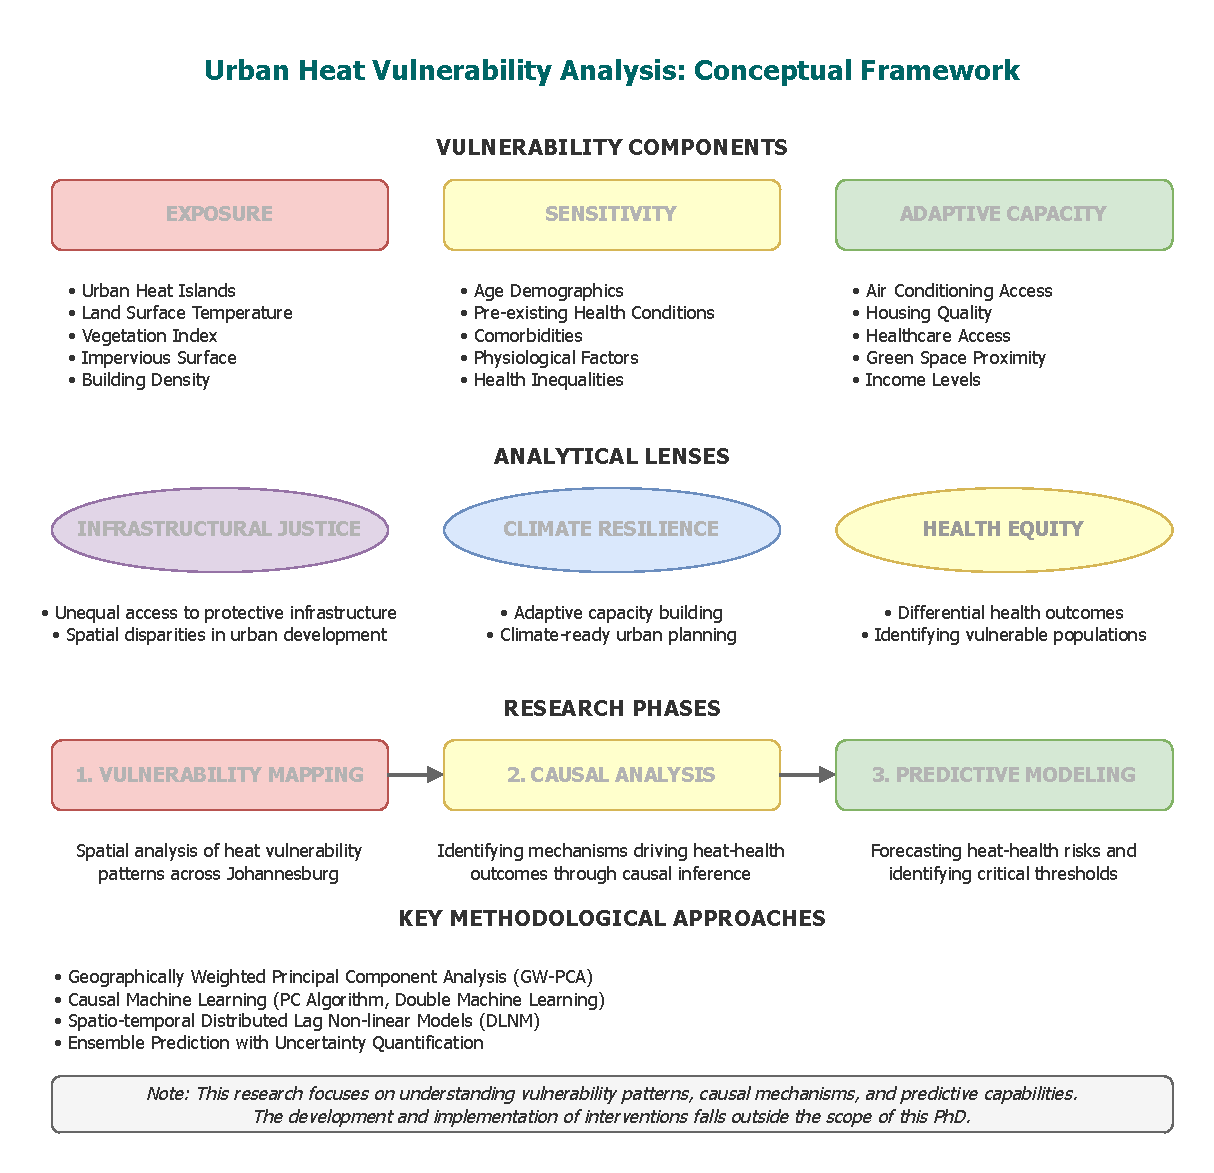
\includegraphics[width=\textwidth]{sections/images/CPframework.drawio.pdf}
\caption{Conceptual framework of urban heat vulnerability analysis showing the three primary dimensions (exposure, sensitivity, adaptive capacity), multiple analytical lenses (infrastructural justice, climate resilience, health equity), and the research phases (vulnerability mapping, causal analysis, predictive modeling). This framework emphasizes how these components interact across Johannesburg's diverse urban landscape while maintaining methodological rigor through geographically weighted approaches.}
\label{fig:conceptual_framework}
\end{figure}

\subsection{Three Interconnected Objectives}
This research is structured around three interconnected objectives:

\subsubsection{Objective 1: Vulnerability Mapping (Descriptive)}
To develop a comprehensive spatial vulnerability assessment using geographically weighted approaches that account for spatial non-stationarity. This objective will identify patterns of heat risk across Johannesburg's diverse urban landscape, examine how historical development patterns shape contemporary vulnerability, and identify priority intervention areas. The mapping will incorporate multiple analytical lenses including infrastructural justice, climate resilience, and health equity to ensure a holistic understanding of vulnerability patterns.

\subsubsection{Objective 2: Heat-Health Dynamics (Explanatory)}
To identify causal mechanisms underlying observed patterns of heat vulnerability through advanced explanatory modeling. This objective involves investigating which biological systems are most affected by heat stress, how these impacts vary across demographic groups, and what socioeconomic factors mediate these effects. The analysis will employ causal machine learning methods to establish robust relationships between environmental exposures and health outcomes while accounting for spatial correlation in the data.

\subsubsection{Objective 3: Predictive Modeling (Predictive)}
To develop predictive models incorporating near-real-time environmental data, meteorological forecasts, and vulnerability factors to predict heat-health risks. This objective includes identifying critical temperature thresholds and neighborhood-specific warning indicators to support short-term emergency response and longer-term adaptation planning. The 1-3 day forecast window has been specifically selected to align with public health intervention timeframes and meteorological forecast reliability.

These three objectives form an integrated research framework addressing spatial, physiological, temporal, and policy dimensions of heat vulnerability. The research design builds each objective upon the findings of the previous one, creating a cohesive pathway from vulnerability characterization to mechanistic understanding to practical solution development.
